
\documentclass{beamer}
\usepackage[utf8]{inputenc}
\usepackage{hyperref}
\usepackage{amsmath}
\usepackage[T1]{fontenc}
\usepackage{centernot}
\usepackage{algpseudocode}
\usepackage{algorithm}
\usepackage{tikz}
\usetikzlibrary{shapes.misc, positioning}
\usetikzlibrary{shapes.geometric, arrows, positioning}
\usepackage{mwe}% for example pictures
\usepackage{xcolor}

\usepackage{latexsym,xcolor,multicol,booktabs,calligra}
\usepackage{amsmath,amssymb,BOONDOX-cal,bm}	
\usepackage{graphicx,pstricks,stackengine}  
\usetheme{Berlin}

\usecolortheme{beaver}

\author{1905091,1905099,1905103}
%\titlegraphic{\includegraphics[width=\textwidth]{unilogo4cmittel.jpg}}


\title{MINIMUM VERTEX COVER}
\subtitle{Beamer Presentation}
\institute[CSE, BUET]
{
  Department of Computer Science and Engineering\\
  Bangladesh University of Engineering and Technology
}
\date{\today}
\logo{\includegraphics[height=1cm]{BUET_LOGO.svg}}

\AtBeginSection[]
{
  \begin{frame}
    \frametitle{Table of Contents}
    \tableofcontents[currentsection]
  \end{frame}
}

\begin{document}

\frame{\titlepage}
\begin{frame}{Table of contents}
    \tableofcontents

\end{frame}

\section{Part 1}

\begin{frame}{Definition}

\begin{alertblock}{The vertex-cover problem}

A vertex cover of an undirected graph G=(V,E) is a subset $V^{'} \subseteq V $ such that if $(u,v) \in E$, then $u \in V^{'}$ or $v \in V{'}$ (or both).\\\\
\newline That is, each vertex “covers” its
incident edges, and a vertex cover for G is a set of vertices that covers all the edges
in E. The size of a vertex cover is the number of vertices in it.

\end{alertblock}

    
\end{frame}

\begin{frame}{Example}

\begin{figure}[h]
  \centering
    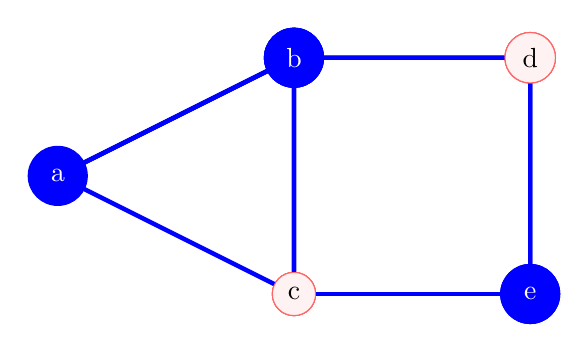
\begin{tikzpicture}[scale=1.5]
      \tikzset{edge/.style = {-,red!60}}
      \tikzset{high_edge/.style = {-, blue,ultra thick}}
      \tikzset{vertex/.style = {shape=circle,draw=red!60, fill=red!5,minimum size=1.5em}}

      %first page
     
      \node[vertex] (a) at (0,1) {a};
      \node[vertex] (b) at (2,2) {b};
      \node[vertex] (c) at (2,0) {c};
      \node[vertex] (d) at (4,2) {d};
      \node[vertex] (e) at (4,0) {e};
      
      \draw[edge] (a) to (b);
      \draw[edge] (b) to (c);
      \draw[edge] (a) to (c);
      \draw[edge] (b) to (d);
      \draw[edge] (c) to (e);
      \draw[edge] (d) to (e);

      %2nd page
     \node[vertex] (a) at (0,1) {a};
      \draw<2>[ fill = blue,draw=blue ,text=white] (2,2) circle (0.25cm) node(b)[]{b};
      \node[vertex] (c) at (2,0) {c};
      \node[vertex] (d) at (4,2) {d};
      \node[vertex] (e) at (4,0) {e};
      
      \draw<2>[high_edge] (a) to (b);
      \draw<2>[high_edge] (b) to (c);
      \draw[edge] (a) to (c);
      \draw<2>[high_edge] (b) to (d);
      \draw[edge] (c) to (e);
      \draw[edge] (d) to (e);

      %3rd page
       \node[vertex] (a) at (0,1) {a};
      \draw<2->[ fill = blue,draw=blue,text=white] (2,2) circle (0.25cm) node(b)[]{b};
      \node[vertex] (c) at (2,0) {c};
      \node[vertex] (d) at (4,2) {d};
      \draw<3->[ fill = blue,draw=blue,text=white] (4,0) circle (0.25cm) node(e)[]{e};
      
      \draw<2->[high_edge] (a) to (b);
      \draw<2->[high_edge] (b) to (c);
      \draw[edge] (a) to (c);
      \draw<2->[high_edge] (b) to (d);
      \draw<3->[high_edge] (c) to (e);
      \draw<3->[high_edge] (d) to (e);

       %4th page
       \draw<4->[ fill = blue,draw=blue,text=white] (0,1) circle (0.25cm) node(a)[]{a};
      \draw<2->[ fill = blue,draw=blue,text=white] (2,2) circle (0.25cm) node(b)[]{b};
      \node[vertex] (c) at (2,0) {c};
      \node[vertex] (d) at (4,2) {d};
      \draw<3->[ fill = blue,draw=blue,text=white] (4,0) circle (0.25cm) node(e)[]{e};
      
      \draw<2->[high_edge] (a) to (b);
      \draw<2->[high_edge] (b) to (c);
      \draw<4->[high_edge] (a) to (c);
      \draw<2->[high_edge] (b) to (d);
      \draw<3->[high_edge] (c) to (e);
      \draw<3->[high_edge] (d) to (e);
      

      
    \end{tikzpicture}
  \caption{Vertex Cover Example}
\end{figure}
    
\end{frame}

\begin{frame}{Minimum vertex cover}

 \only<1>{\begin{alertblock}{Problem statement}
      The vertex-cover problem is to find a vertex cover of minimum size in a given
graph. Restating this optimization problem as a decision problem, we wish to determine whether a graph has a vertex cover of a given size k. As a language, we
define\\  VERTEX-COVER=\{<G,K> : graph G has a vertex cover of size k\}
   \end{alertblock}}
    
\end{frame}

\begin{frame}{Vertex Cover Problem is NP Copmplete}

    \begin{alertblock}{Statement}

The vertex cover problem is an NP-Complete problem, which means that there is no known polynomial-time solution for finding the minimum vertex cover of a graph unless it can be proven that\\ P = NP. 
\end{alertblock}

\end{frame}

\begin{frame}{Proof}\transdissolve
\only<1>{\begin{alertblock}{Vertex cover $\in NP$}
  Suppose we are given a graph G=(V,E) and an integer $k$. Let $V^{'} \subseteq V$ and $|V^{'}|=k$. Then it checks for each edge $(u,v) \in E , $ that $u\in V^{'}$ or $v \in V^{'}$. We can easily verify the certificate in polynomial time.
   \end{alertblock} }
  \only<2>{\begin{alertblock}{Vertex cover $\in NP$ hard}
  In order to prove that Vertex cover is an NP-hard problem we reduce a known NP-hard problem to vertex cover problem. We chose clique for an instance.
   \end{alertblock}}

   \only<3>{\begin{alertblock}{Complement graph}
       Given a graph G=(V,E) we define complement of G as $\Bar{G}$=(V,$\Bar{E}$),
       Where $\Bar{E}$=\{(u,v):u,v$\in$ V,u $\centernot \subseteq v$ and (u,v) $\centernot\in$ E\}
   \end{alertblock}}

   \only<4>{\begin{alertblock}{Reduction algorithm}
       The reduction algorithm takes as input an instance (G,K) of the clique problem .\\
       It computes the complement $\Bar{G}$ in polynomial time. ($\Bar{G},|V|-K$) is an instance of vertex cover problem. 
   \end{alertblock}}
   \only<4>{\begin{alertblock}{Reduced problem}
       The graph G has a clique of size k if and only if the graph $\Bar{G}$ has a vertex cover of size |V|-k
   \end{alertblock}}

   
\begin{columns}

\column{0.5\linewidth}
    
\begin{figure}
    \centering
    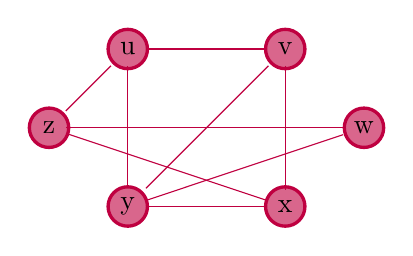
\begin{tikzpicture}
     \tikzset{edge/.style = {-,red!60}}
      \tikzset{high_edge/.style = {-, blue,ultra thick}}
      \tikzset{vertex/.style = {shape=circle,draw=purple, fill=purple!60,very thik,minimum size=1.5em}}
      
        \draw<3,5> [ fill = purple!60,draw=purple,very thick] (4,4) circle (0.25cm) node(z)[]{z};
        \draw<3,5>[ fill = purple!60,draw=purple,very thick] (5,5) circle (0.25cm) node(u)[]{u};
        \draw<3,5>[ fill = purple!60,draw=purple,very thick] (5,3) circle (0.25cm) node(y)[]{y};
        \draw<3,5>[ fill = purple!60,draw=purple,very thick] (7,5) circle (0.25cm) node(v)[]{v};
        \draw<3,5>[ fill = purple!60,draw=purple,very thick] (7,3) circle (0.25cm) node(x)[]{x};
        \draw<3,5> [ fill = purple!60,draw=purple,very thick] (8,4) circle (0.25cm) node(w)[]{w};
            
        
        \draw<3,5> [-,purple] (z) -- (u);
        \draw<3,5> [-,purple] (z) -- (x);
        \draw<3,5> [-,purple] (z) -- (w);
        \draw<3,5> [-,purple] (y) -- (u);
        \draw<3,5> [-,purple] (y) -- (v);
        \draw<3,5> [-,purple] (y) -- (w);
        \draw<3,5> [-,purple] (y) -- (x);
        \draw<3,5> [-,purple] (u) -- (v);
        \draw<3,5> [-,purple] (v) -- (x);
        % \draw<3,5> [-,blue,ultra thick] (u) -- (x);
        % \draw<3,5> [-,blue,ultra thick] (z) -- (v);
        % \draw<3,5> [-,blue,ultra thick] (v) -- (w);
        % \draw<3,5> [-,blue,ultra thick] (x) -- (w);
        % \draw<3,5> [-,blue,ultra thick] (y) -- (z);
        

       
    \end{tikzpicture}
   \only<3,5>{
   \caption{G}
   }
    \label{fig:g1}
\end{figure}

\column{0.5\linewidth}

\begin{figure}
    \centering
    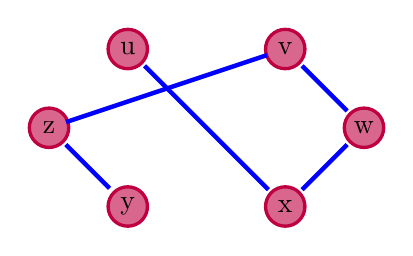
\begin{tikzpicture}
     \tikzset{edge/.style = {-,red!60}}
      \tikzset{high_edge/.style = {-, blue,ultra thick}}
      \tikzset{vertex/.style = {shape=circle,draw=purple, fill=purple!60,very thik,minimum size=1.5em}}
      
        \draw<3,5> [ fill = purple!60,draw=purple,very thick] (4,4) circle (0.25cm) node(z)[]{z};
        \draw<3,5>[ fill = purple!60,draw=purple,very thick] (5,5) circle (0.25cm) node(u)[]{u};
        \draw<3,5>[ fill = purple!60,draw=purple,very thick] (5,3) circle (0.25cm) node(y)[]{y};
        \draw<3,5>[ fill = purple!60,draw=purple,very thick] (7,5) circle (0.25cm) node(v)[]{v};
        \draw<3,5>[ fill = purple!60,draw=purple,very thick] (7,3) circle (0.25cm) node(x)[]{x};
        \draw<3,5> [ fill = purple!60,draw=purple,very thick] (8,4) circle (0.25cm) node(w)[]{w};
            
        
        \draw<3,5> [-,blue,ultra thick] (u) -- (x);
        \draw<3,5> [-,blue,ultra thick] (z) -- (v);
        \draw<3,5> [-,blue,ultra thick] (v) -- (w);
        \draw<3,5> [-,blue,ultra thick] (x) -- (w);
        \draw<3,5> [-,blue,ultra thick] (y) -- (z);
       
       
    \end{tikzpicture}
    \only<3,5>{
   \caption{$\Bar{G}$}
   }
    \label{fig:g2}
\end{figure}


\end{columns}
   \only<5>{\alert{
       The graph G has a clique of size k if and only if the graph $\Bar{G}$ has a vertex cover of size |V|-k
}}

\end{frame}





\section{Part 2}
\begin{frame}{Optimal solution?}
\textbf{\large Naive approach}\\
We can naively solve the problem by iterating over all the subsets of the vertices and using only those vertices, forming a new graph containing all the edges contained by these vertices. Then we can check if this new graph, contains all the edges of the original graph or not based on which it can be a candidate for the vertex cover. Out of all the candidates, we print the set, which has the minimum size.\\

This naive approach will have an exponential runtime complexity.
    
    
\end{frame}

\begin{frame}{Approximation}\transdissolve
\only<1>{
\begin{alertblock}{Some hope?}

Even though we do not know how to find an optimal vertex cover in a graph G in polynomial time, we can efficiently find a vertex cover that is near optimal.

\end{alertblock}
}



\only<2>{\begin{alertblock}{Definition}

An approximation algorithm for a problem is a polynomial-time algorithm that, when given input i, outputs an element of FS(i), which is the set of feasible solutions for i.

\end{alertblock}}
\only<2>{\begin{alertblock}{Approach}

The following approximation algorithm takes as input an undirected graph G and
returns a vertex cover whose size is guaranteed to be no more than twice the size
of an optimal vertex cover.
\end{alertblock}}
  

\end{frame}

\begin{frame}[fragile]{Approximate Vertex Cover}
\begin{algorithmic}[1]
  \Require{A graph $G=(V,E)$}
  \Ensure{A vertex cover $C\subseteq V$}
  \State $C \gets \emptyset$
  \For{$(u,v) \in E$}
    \If{$u \notin C$ and $v \notin C$}
      \State $C \gets C \cup \{u\}$
      \State $C \gets C \cup \{v\}$
    \EndIf
  \EndFor
  \State \Return{$C$}
\end{algorithmic}
\end{frame}


\begin{frame}{Approx algorithm continued....}
\begin{columns}

\column{0.5\linewidth}

\tikzstyle{vertex} = [circle, radius = 3 cm, text centered]

\tikzstyle{arrow}=[thick,-,>=stealth,draw=purple]
\begin{tikzpicture}

\node<1> (Node1)[vertex, draw =purple!80, ,fill=purple!50 ] {\textcolor{white}{1}};
\node<1> (Node2)[vertex,right of=Node1, draw =purple!80, ,fill=purple!50 ] {\textcolor{white}{2}};
\node<1> (Node3)[vertex, right of=Node2, draw=purple!80, ,fill=purple!50] {\textcolor{white}{3}};
\node<1> (Node4)[vertex,below of=Node1, draw =purple!80, ,fill=purple!50] {\textcolor{white}{4}};
\node<1> (Node5)[vertex ,below of=Node2, draw =purple!80, ,fill=purple!50] {\textcolor{white}{5}};
\node<1> (Node6)[vertex,below of=Node3 , draw =purple!80, ,fill=purple!50 ] {\textcolor{white}{6}};
\node<1> (Node8)[vertex ,right of=Node3] {\textcolor{white}{7}};
\node<1> (Node7)[vertex,below of=Node8, draw =purple!80, ,fill=purple!50] {\textcolor{white}{8}};


\draw<1> [arrow] (Node1)--(Node2);
\draw<1> [arrow,] (Node2)--(Node3);
\draw<1> [arrow] (Node1)--(Node4);
\draw<1> [arrow] (Node2)--(Node5);
\draw<1> [arrow] (Node5)--(Node6);
\draw<1> [arrow] (Node6)--(Node3);
\draw<1> [arrow] (Node7)--(Node3);
\draw<1> [arrow] (Node5)--(Node3);

\end{tikzpicture}

\begin{tikzpicture}[scale=4]

\node<2> (Node1)[vertex, draw =blue!80, ,fill=blue!50 ] {\textcolor{white}{1}};
\node<2> (Node2)[vertex,right of=Node1, draw =blue!80, ,fill=blue!50 ] {\textcolor{white}{2}};
\node<2> (Node3)[vertex, right of=Node2, draw=purple!80, ,fill=purple!50] {\textcolor{white}{3}};
\node<2> (Node4)[vertex,below of=Node1, draw =purple!80, ,fill=purple!50] {\textcolor{white}{4}};
\node<2> (Node5)[vertex ,below of=Node2, draw =purple!80, ,fill=purple!50] {\textcolor{white}{5}};
\node<2> (Node6)[vertex,below of=Node3 , draw =purple!80, ,fill=purple!50 ] {\textcolor{white}{6}};
\node<2> (Node8)[vertex ,right of=Node3] {\textcolor{white}{7}};
\node<2> (Node7)[vertex,below of=Node8, draw =purple!80, ,fill=purple!50] {\textcolor{white}{8}};


\draw<2> [arrow,ultra thick,blue] (Node1)--(Node2);
\draw<2> [arrow,dashed] (Node2)--(Node3);
\draw<2> [arrow,dashed] (Node1)--(Node4);
\draw<2> [arrow,dashed] (Node2)--(Node5);
\draw<2> [arrow] (Node5)--(Node6);
\draw<2> [arrow] (Node6)--(Node3);
\draw<2> [arrow] (Node7)--(Node3);
\draw<2> [arrow] (Node5)--(Node3);

\end{tikzpicture}

\begin{tikzpicture}[scale=4]

\node<3> (Node1)[vertex, draw =blue!80, ,fill=blue!50 ] {\textcolor{white}{1}};
\node<3> (Node2)[vertex,right of=Node1, draw =blue!80, ,fill=blue!50 ] {\textcolor{white}{2}};
\node<3> (Node3)[vertex, right of=Node2, draw=purple!80, ,fill=purple!50] {\textcolor{white}{3}};
\node<3> (Node4)[vertex,below of=Node1, draw =purple!80, ,fill=purple!50] {\textcolor{white}{4}};
\node<3> (Node5)[vertex ,below of=Node2, draw =blue!80, ,fill=blue!50] {\textcolor{white}{5}};
\node<3> (Node6)[vertex,below of=Node3 , draw =blue!80, ,fill=blue!50 ] {\textcolor{white}{6}};
\node<3> (Node8)[vertex ,right of=Node3] {\textcolor{white}{7}};
\node<3> (Node7)[vertex,below of=Node8, draw =purple!80, ,fill=purple!50] {\textcolor{white}{8}};


\draw<3> [arrow] (Node1)--(Node2);
\draw<3> [arrow,dashed] (Node2)--(Node3);
\draw<3> [arrow,dashed] (Node1)--(Node4);
\draw<3> [arrow,dashed] (Node2)--(Node5);
\draw<3> [arrow] (Node5)--(Node6);
\draw<3> [arrow,dashed] (Node6)--(Node3);
\draw<3> [arrow] (Node7)--(Node3);
\draw<3> [arrow,dashed] (Node5)--(Node3);

\end{tikzpicture}



\begin{tikzpicture}[scale=4]

\node<4> (Node1)[vertex, draw =blue!80, ,fill=blue!50 ] {\textcolor{white}{1}};
\node<4> (Node2)[vertex,right of=Node1, draw =blue!80, ,fill=blue!50 ] {\textcolor{white}{2}};
\node<4> (Node3)[vertex, right of=Node2, draw=blue!80, ,fill=blue!50] {\textcolor{white}{3}};
\node<4> (Node4)[vertex,below of=Node1, draw =purple!80, ,fill=purple!50] {\textcolor{white}{4}};
\node<4> (Node5)[vertex ,below of=Node2, draw =blue!80, ,fill=blue!50] {\textcolor{white}{5}};
\node<4> (Node6)[vertex,below of=Node3 , draw =blue!80, ,fill=blue!50 ] {\textcolor{white}{6}};
\node<4> (Node8)[vertex ,right of=Node3] {\textcolor{white}{7}};
\node<4> (Node7)[vertex,below of=Node8, draw =blue!80, ,fill=blue!50] {\textcolor{white}{8}};


\draw<4> [arrow] (Node1)--(Node2);
\draw<4> [arrow,dashed] (Node2)--(Node3);
\draw<4> [arrow,dashed] (Node1)--(Node4);
\draw<4> [arrow,dashed] (Node2)--(Node5);
\draw<4> [arrow,dashed] (Node5)--(Node6);
\draw<4> [arrow,dashed] (Node6)--(Node3);
\draw<4> [arrow] (Node7)--(Node3);
\draw<4> [arrow,dashed] (Node5)--(Node3);

\end{tikzpicture}

\begin{tikzpicture}[scale=4]

\node<5> (Node1)[vertex, draw =blue!80, ,fill=blue!50 ] {\textcolor{white}{1}};
\node<5> (Node2)[vertex,right of=Node1, draw =blue!80, ,fill=blue!50 ] {\textcolor{white}{2}};
\node<5> (Node3)[vertex, right of=Node2, draw=blue!80, ,fill=blue!50] {\textcolor{white}{3}};
\node<5> (Node4)[vertex,below of=Node1, draw =purple!80, ,fill=purple!50] {\textcolor{white}{4}};
\node<5> (Node5)[vertex ,below of=Node2, draw =blue!80, ,fill=blue!50] {\textcolor{white}{5}};
\node<5> (Node6)[vertex,below of=Node3 , draw =blue!80, ,fill=blue!50 ] {\textcolor{white}{6}};
\node<5> (Node8)[vertex ,right of=Node3] {\textcolor{white}{7}};
\node<5> (Node7)[vertex,below of=Node8, draw =blue!80, ,fill=blue!50] {\textcolor{white}{8}};


\draw<5> [arrow] (Node1)--(Node2);
\draw<5> [arrow] (Node2)--(Node3);
\draw<5> [arrow] (Node1)--(Node4);
\draw<5> [arrow] (Node2)--(Node5);
\draw<5> [arrow] (Node5)--(Node6);
\draw<5> [arrow] (Node6)--(Node3);
\draw<5> [arrow] (Node7)--(Node3);
\draw<5> [arrow] (Node5)--(Node3);

\end{tikzpicture}

\begin{tikzpicture}[scale=4]

\node<6> (Node1)[vertex, draw =blue!80, ,fill=blue!50 ] {\textcolor{white}{1}};
\node<6> (Node2)[vertex,right of=Node1, draw =purple!80, ,fill=purple!50 ] {\textcolor{white}{2}};
\node<6> (Node3)[vertex, right of=Node2, draw=blue!80, ,fill=blue!50] {\textcolor{white}{3}};
\node<6> (Node4)[vertex,below of=Node1, draw =purple!80, ,fill=purple!50] {\textcolor{white}{4}};
\node<6> (Node5)[vertex ,below of=Node2, draw =blue!80, ,fill=blue!50] {\textcolor{white}{5}};
\node<6> (Node6)[vertex,below of=Node3 , draw =purple!80, ,fill=purple!50 ] {\textcolor{white}{6}};
\node<6> (Node8)[vertex ,right of=Node3] {\textcolor{white}{7}};
\node<6> (Node7)[vertex,below of=Node8, draw =purple!80, ,fill=purple!50] {\textcolor{white}{8}};


\draw<6> [arrow] (Node1)--(Node2);
\draw<6> [arrow] (Node2)--(Node3);
\draw<6> [arrow] (Node1)--(Node4);
\draw<6> [arrow] (Node2)--(Node5);
\draw<6> [arrow] (Node5)--(Node6);
\draw<6> [arrow] (Node6)--(Node3);
\draw<6> [arrow] (Node7)--(Node3);
\draw<6> [arrow] (Node5)--(Node3);

\end{tikzpicture}




\end{columns}



\end{frame}


\section{Part 3}
\begin{frame}{Efficiency}
   We can see that approximation does not always give a minimum vertex cover, but it can be proven that the returned vertex cover is at most twice the size of an optimal cover.
\end{frame}

\begin{frame}{Proof}
    Let $A$ denote the set of edges that line $4$ of APPROX VERTEX COVER picked. In order to cover the edges in $A$,
    \begin{itemize}
        \item an optimal cover C* must include at least one endpoint of each edge in A.\\
        \item No two edges of A share an endpoint.\\
    \end{itemize}
\end{frame}

\begin{frame}{Proof}
    \begin{alertblock}{Lower  Bound}
        |C*|>=|A|
    \end{alertblock}
\end{frame}

\begin{frame}{Proof}
    Each execution of line 4 picks an edge for which neither of its endpoints is already in $C$, yielding 
    \begin{alertblock}{Upper Bound}
        |C|=2|A|
    \end{alertblock}
\end{frame}

\begin{frame}{Proof}
    Combining we get, 
    \begin{alertblock}{Conclusion}
        |C|=2|A|
        =>|C|<=2|C*|
    \end{alertblock}
\end{frame}

\section{Conclusion}
\begin{frame}{Key Points}
    \begin{itemize}
        \item A set of minimum number of vertices such that each edge of the graph is incident to at least one vertex of the set, is called the vertex cover.\\ \pause
        \item Although minimum vertex cover is a NP hard problem, near optimal solution can be found in polynomial time.\\ \pause
        \item While greedy algorithm might not be optimal, approximation algorithm guarantees a near optimal solution.\\ 
    \end{itemize}
\end{frame}

\end{document}
